% This file was created by tikzplotlib v0.9.8.
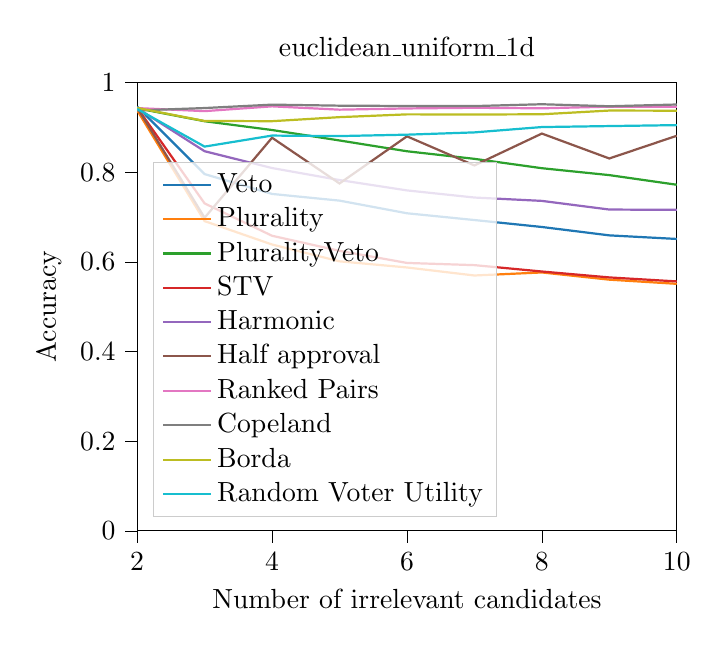
\begin{tikzpicture}

\definecolor{color0}{rgb}{0.12156862745098,0.466666666666667,0.705882352941177}
\definecolor{color1}{rgb}{1,0.498039215686275,0.0549019607843137}
\definecolor{color2}{rgb}{0.172549019607843,0.627450980392157,0.172549019607843}
\definecolor{color3}{rgb}{0.83921568627451,0.152941176470588,0.156862745098039}
\definecolor{color4}{rgb}{0.580392156862745,0.403921568627451,0.741176470588235}
\definecolor{color5}{rgb}{0.549019607843137,0.337254901960784,0.294117647058824}
\definecolor{color6}{rgb}{0.890196078431372,0.466666666666667,0.76078431372549}
\definecolor{color7}{rgb}{0.737254901960784,0.741176470588235,0.133333333333333}
\definecolor{color8}{rgb}{0.0901960784313725,0.745098039215686,0.811764705882353}

\begin{axis}[
legend cell align={left},
legend style={
  fill opacity=0.8,
  draw opacity=1,
  text opacity=1,
  at={(0.03,0.03)},
  anchor=south west,
  draw=white!80!black
},
tick align=outside,
tick pos=left,
title={euclidean\_uniform\_1d},
x grid style={white!69.0196078431373!black},
xlabel={Number of irrelevant candidates},
xmin=2, xmax=10,
xtick style={color=black},
y grid style={white!69.0196078431373!black},
ylabel={Accuracy},
ymin=0, ymax=1,
ytick style={color=black}
]
\addplot [thick, color0]
table {%
2 0.9463
3 0.7957
4 0.7514
5 0.7365
6 0.7083
7 0.6932
8 0.6777
9 0.659
10 0.651
};
\addlegendentry{Veto}
\addplot [thick, color1]
table {%
2 0.9381
3 0.6908
4 0.6386
5 0.6011
6 0.5874
7 0.5695
8 0.5763
9 0.5602
10 0.5509
};
\addlegendentry{Plurality}
\addplot [thick, color2]
table {%
2 0.9424
3 0.9136
4 0.894
5 0.8707
6 0.8466
7 0.8297
8 0.8088
9 0.7934
10 0.7719
};
\addlegendentry{PluralityVeto}
\addplot [thick, color3]
table {%
2 0.9439
3 0.7303
4 0.6581
5 0.6245
6 0.5975
7 0.5926
8 0.5784
9 0.5652
10 0.5563
};
\addlegendentry{STV}
\addplot [thick, color4]
table {%
2 0.9428
3 0.8467
4 0.8092
5 0.7824
6 0.7593
7 0.7434
8 0.7359
9 0.7166
10 0.7159
};
\addlegendentry{Harmonic}
\addplot [thick, color5]
table {%
2 0.9441
3 0.6983
4 0.8768
5 0.7748
6 0.8799
7 0.815
8 0.8861
9 0.8305
10 0.8812
};
\addlegendentry{Half approval}
\addplot [thick, color6]
table {%
2 0.9429
3 0.9361
4 0.9468
5 0.9394
6 0.9421
7 0.9436
8 0.9424
9 0.9461
10 0.946
};
\addlegendentry{Ranked Pairs}
\addplot [thick, white!49.8039215686275!black]
table {%
2 0.9376
3 0.943
4 0.9506
5 0.9483
6 0.9476
7 0.9474
8 0.9515
9 0.947
10 0.9509
};
\addlegendentry{Copeland}
\addplot [thick, color7]
table {%
2 0.9433
3 0.9141
4 0.9137
5 0.9227
6 0.9289
7 0.9286
8 0.9291
9 0.9374
10 0.9371
};
\addlegendentry{Borda}
\addplot [thick, color8]
table {%
2 0.9409
3 0.857
4 0.8816
5 0.8805
6 0.8836
7 0.8887
8 0.9006
9 0.9028
10 0.9049
};
\addlegendentry{Random Voter Utility}
\end{axis}

\end{tikzpicture}
